%==================================================================FRONT PAGE AND TOC
% For article only
\mode<presentation:0>{\thispagestyle{empty}\maketitle}

% For presentation only
\mode<presentation| article:0| handout:0>{
    \begin{frame}<article:0>[label=portada]
    \titlepage
    \end{frame}%Fin del frame
}

% For handout only
\mode<handout>{
  \begin{frame}[label=portada]
    \maketitle
  \end{frame}
}

% %% TABLE OF CONTENTS
% \begin{frame}[label=toc]
%     \mode<article:0>{\frametitle{Contents}}
%     \mode<presentation>{\small}
%     \tableofcontents[hidesubsections]
% \end{frame}

\begin{frame}[label=portada]
 \titlepage
\end{frame}
\begin{frame}[label=toc]
  \frametitle{Resumen}
\tableofcontents[hidesubsections]
\end{frame}
% \rowcolors{1}{ZurichBlue!20}{ZurichBlue!5}
%%==================================================================S INTRODUCTION
\section{Software Libre}
%%==================================================================F 
\begin{frame}
  \frametitle{Qué es Software Libre?}
  \begin{itemize}
    \item 4 Libertades esenciales:
    \begin{enumerate}
      \setcounter{enumi}{-1}
      \item Libertad de \alert{usar} el programa, con cualquier propósito
      \item Libertad de \alert{estudiar} cómo funciona el programa y \alert{modificarlo}, adaptándolo a tus necesidades.
      \item Libertad de \alert{distribuir copias} del programa, con lo cual puedes ayudar a tu prójimo.
      \item Libertad de \alert{mejorar} el programa y \alert{hacer públicas} esas mejoras a los demás, de modo que toda la comunidad se beneficie. 
    \end{enumerate}
    \item Las \alert{Libertades 1} y \alert{3} requieren acceso al código fuente
    \item La \alert{Libertad 0} nos permite tener el control sobre nuestra informatica
    \item La \alert{Libertad 2} nos permite ayudar a nuestro prójimo
  \end{itemize}
\end{frame}
%%==================================================================F 
\begin{frame}
  \frametitle{Libre vs. Abierto vs. Gratis vs. Privativo}
  \begin{itemize}
    \item El término inglés \alert{\emph{free}} es ambiguo:
    \begin{itemize}
      \item Libre (\emph{Freedom of speach} o libertad de expresión)
      \item Gratis (\emph{Free Beer!} o Cerveza gratis!)
    \end{itemize}
    \item Gratis \alert{$\ne$} Libre $\Rightarrow$ \alert{Gratis} hace referencia al precio
    \item Libre \alert{$\ne$} Abierto
    \begin{itemize}
      \item \alert{Abierto} hace referencia al que el código es público
      \item \alert{Libre} hace referencia a la libertad de uso y disponibilidad del software y su código
    \end{itemize}
    \item El \alert{software privativo} o \alert{proprietario}, el código es cerrado, su uso está limitado, generalmente se pagan grandes cantidades de dinero para su licenciamiento.
  \end{itemize}
\end{frame}
%%==================================================================F 
\begin{frame}
  \frametitle{Licencias}
  \begin{itemize}
    \item Libres y permisivas
    \begin{itemize}
      \item \alert{GPL}: General Public License. Licencia Libre
      \item \alert{LPGL}: Lesser General Public License. Licencia permisiva que permite el uso del código fuente en software no libre
      \item \alert{BSD}: Berkeley Software Distribution. Licencia permisiva que permite el uso del código fuente en software no libre
      \item \alert{MIT}: Massachusetts Institute of Technology License. Licencia permisiva.
    \end{itemize}
    \item \alert{Proprietarias}: Requiere permiso expreso del titular del software
    \item \alert{Freeware}: Sin costo, disponible para su uso y por tiempo ilimitado
    \item \alert{Shareware}: Evaluación gratuita con limitaciones: tiempo y/o capacidades
  \end{itemize}
\end{frame}
%%==================================================================S INTRODUCTION
\section{Software proprietario}
%%==================================================================F 
\begin{frame}
  \frametitle{Software proprietarios y no cerrados}
  \begin{itemize}
    \item Terrascan y Terrasolid
      \begin{itemize}
       \item Actualmente el más usado
       \item Es un CAD
       \item Proprietario
      \end{itemize}
    \item ArcGIS
      \begin{itemize}
        \item Cada vez más utilizado
        \item Es un GIS
       \item Proprietario
      \end{itemize}
    \item Scop++ y OPALS 
    \begin{itemize}
      \item Universidad TU Wien
      \item Proprietario
      \item \beamergotobutton{\url{http://photo.geo.tuwien.ac.at/software/scop/}}
    \end{itemize}
    \item FUSION 
    \begin{itemize}
      \item Aplicaciones forestales
      \item Cerrado
      \item \beamergotobutton{\url{http://forsys.cfr.washington.edu/JFSP06/lidar_&_ifsar_tools.htm}}
    \end{itemize}
  \end{itemize}
\end{frame}
%%==================================================================S INTRODUCTION
\section{Herramientas libres y abiertas}
%%==================================================================F 
\begin{frame}
  \frametitle{Herramientas}
  \begin{enumerate}
    \item GRASS LiDAR tools 
    	\begin{itemize}
        \item \texttt{v.outlier}, \texttt{v.lidar.edgedetetion}, \texttt{v.lidar.growing}, \texttt{v.lidar.correction}, \texttt{v.surf.bspline}
    	\end{itemize}
    \item LibLAS
    	\begin{itemize}
        \item \texttt{las2las}, \texttt{las2txt}, \texttt{txt2las}, \texttt{lasdiff}, \texttt{lasinfo} 
    	\end{itemize}
    \item LAStools
    	\begin{itemize}
        \item \texttt{las2las}, \texttt{las2txt}, \texttt{txt2las}, \texttt{shp2las}, \texttt{lasground}, \texttt{las2dem}, \texttt{txt2tin}
    	\end{itemize}
    \item SPDlib (Sorted Pulse Data Library)
      \begin{itemize}
        \item \texttt{spdtranslate}, \texttt{spdrmnoise}, \texttt{spdpmfgrd}, \texttt{spdmccgrd}, \texttt{spddefheight}, \texttt{spdinterp}, \texttt{spdmetrics}
      \end{itemize}
    \item PDAL (Point Data Abstraction Library)
    \item PCL (Point Cloud Library)
  \end{enumerate}
\end{frame}
%%==================================================================Sb
\subsection{Análisis LiDAR en GRASS}
%%==================================================================F
\begin{frame}
    \frametitle{Geographic Resources Analysis Support System\hfill
        
\includegraphics[width=0.7cm]{images/grasslogo_transp_big.png}} 
     \begin{itemize}
        \item Conocido como \alert<1>{GRASS}: GIS para manipulación y
            análisis de datos geoespaciales.
        \item Como es un programa de \alert{códico abierto} con un montón de
            librerias, es muy adecuado para la implementación de nuestras
            propias herramientas.
        \item Escrito en C/C++, lo que permite implementar programas
            computacionalmente pesados $\Rightarrow$ \alert{ideal} para trabajar
            con LiDAR.
        \item GRASS $\geq$ 6 incluye indexación topológica $\Rightarrow$
            \alert{fatal} para trabajar con LiDAR.  \item Hay versiones para
            GNU/Linux, MS-Windows, Mac-OSX, SUN, etc.
            \alert{\textexclamdown\textexclamdown Todos lo pueden utilizar!!}
        \item Más información en:
            \beamergotobutton{\url{http://grass.osgeo.ogr}}
    \end{itemize}
\end{frame}
% %%==================================================================Sb
% \subsubsection{Importando nube de puntos}
% %%==================================================================F 
% \begin{frame}
%  \frametitle{Importar como raster: \LARGE\path{r.in.xyz}}
% \end{frame}
% %%==================================================================F 
% \begin{frame}
%  \frametitle{Importar como vectorial: \LARGE\path{v.in.ascii}}
% \end{frame}
%%==================================================================F 
\begin{frame}
  \frametitle{Herramientas LiDAR de GRASS}
  Eliminación de objetos en nubes de puntos y creación de MDT's
  \begin{minipage}{0.45\textwidth}
  \begin{itemize}
    \item<1-> \path{v.in.las}
    \item<2-> \path{v.outlier}
    \item<3-> \path{v.lidar.edgedetection}
    \item<4-> \path{v.lidar.growing}
    \item<5-> \path{v.lidar.correction}
    \item<6-> \path{v.surf.bspline}
  \end{itemize}
  \end{minipage}
  \begin{minipage}{0.45\textwidth}
    \begin{picture}(275,110)
    \uncover<3->{\put(0,0){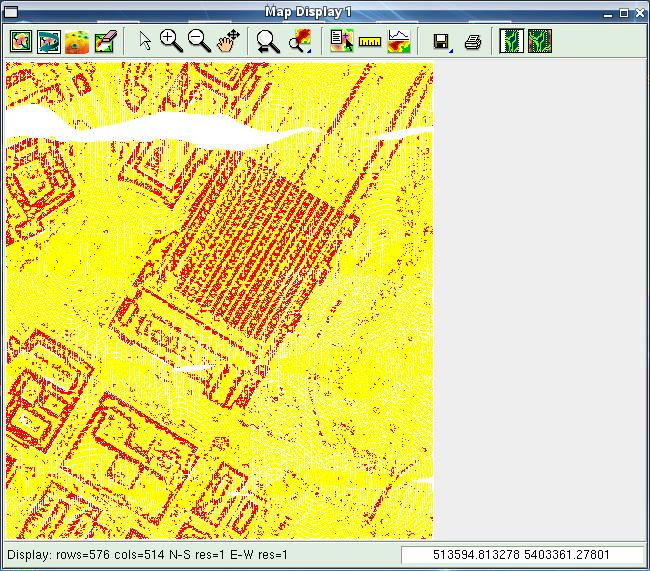
\includegraphics[width=0.75\textwidth]{images/edge}}}
    \uncover<4->{\put(10,-10){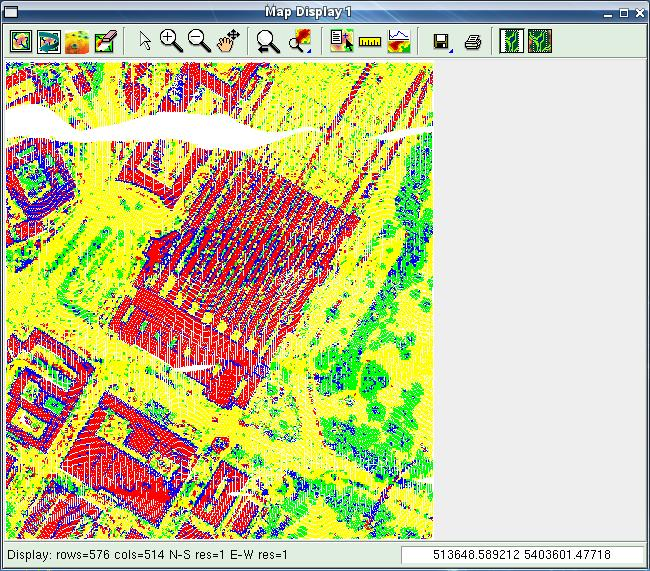
\includegraphics[width=0.75\textwidth]{images/grow}}}
    \uncover<5->{\put(20,-20){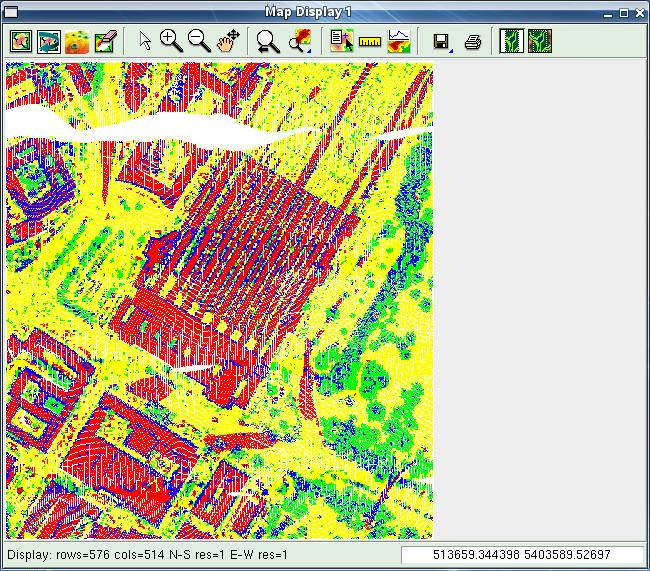
\includegraphics[width=0.75\textwidth]{images/correction}}}
    \end{picture}
  \end{minipage}
\end{frame}
%%==================================================================Sb
\subsubsection{\texttt{v.outlier}}
%%==================================================================F 
\begin{frame}[fragile,shrink=5]
  \frametitle{\path{v.outlier}}
  \begin{beamerboxesrounded}[shadow=true]{\textbf{\path{v.lidar.edgedetection}}
    \texttt{ input=name output=name outlier=name [soe=value] [son=value] 
    [lambda\_i=value] [thres\_o=value]}}
    \begin{itemize}
      \item \textbf{input}: name of the input vector map
      \item \textbf{output}: name of the output vector map
      \item \textbf{soe}: Interpolation spline step value in e-w direction
      \item \textbf{son}: Interpolation spline step value in n-s direction
      \item \textbf{lambda\_i}: Thychonov regularization weigth. (default: 0.1)
      \item \textbf{thres\_o}: Threshold for the outliers. (default: 50)
    \end{itemize}
  \end{beamerboxesrounded}
  %\pause
  \begin{beamerboxesrounded}[shadow=true]{Sintaxis}
\scriptsize
%\testcode
\begin{verbatim}
GRASS6 (stuttgart): > # Limpiamos el primer impulso
GRASS6 (stuttgart): > v.outlier in=stuttgart_first out=station_first \
> outlier=station_first_out soe=10 son=10 thres_o=25
GRASS6 (stuttgart): > # Limpiamos el ultimo impulso
GRASS6 (stuttgart): > v.outlier in=stuttgart_last out=station_last \
> outlier=station_last_out soe=10 son=10 thres_o=30
\end{verbatim}
\end{beamerboxesrounded}
\end{frame}
%%==================================================================Sb
\subsubsection{\texttt{v.lidar.edgedetection}}
%%==================================================================F 
\begin{frame}[fragile,shrink=10]
  \frametitle{\path{v.lidar.edgedetection}}
  \begin{beamerboxesrounded}[shadow=true]{\textbf{\path{v.lidar.edgedetection}}
    \texttt{ input=name output=name first=name see=value sen=value 
    [lambda\_g=value] [tgh=value] [tgl=value] [theta\_g=value] [lambda\_r=value]}}
   \begin{itemize}
    \item \textbf{input}: name of the input vector map
    \item \textbf{output}: name of the output vector map
    \item \textbf{see}: Interpolation spline step value in e-w direction
    \item \textbf{sen}: Interpolation spline step value in n-s direction
    \item \textbf{lambda\_g}: Regularization weight in gradient evaluation (default: 0.01)
    \item \textbf{tgh}: High gradient threshold for edge classification (default: 6)
    \item \textbf{tgl}: Low gradient threshold for edge classification (default: 3)
    \item \textbf{theta\_g}: Angle range for same direction detection (default: 0.26)
    \item \textbf{lambda\_r}: Regularization weight in residual evaluation (default: 2)
   \end{itemize}
  \end{beamerboxesrounded}
 %\pause
 \begin{beamerboxesrounded}[shadow=true]{Sintaxis}
\scriptsize
%\testcode
\begin{verbatim}
GRASS6 (stuttgart): > v.lidar.edgedetection in=station_last see=4 sen=4 \
> lambda_g=0.1 out=station_edge
\end{verbatim}
\end{beamerboxesrounded}
\end{frame}
%%==================================================================F 
%\pgfdeclareimage[width=0.65\textwidth]{edge}{images/edge}
%\begin{frame}
% \frametitle{Visualización de \LARGE\path{v.lidar.edgedetection}}
%\begin{columns}
%  \begin{column}{0.7\textwidth}
%    \begin{center}
%	\begin{tikzpicture}
%    	  \pgftext[bottom,left,at={\pgfpointxy{0}{0}}]{\pgfuseimage{edge}}
%	\end{tikzpicture}
%   \end{center}
%  \end{column}
%  \begin{column}{0.25\textwidth}
%	\begin{enumerate}
%	 \item \textcolor{red}{Borde}
%	 \item \textcolor{yellow!95!black}{Terreno}
%	\end{enumerate}
%  \end{column}
%\end{columns}
%\end{frame}
%%==================================================================Sb
\subsubsection{\texttt{v.lidar.growing}}
%%==================================================================F 
\begin{frame}[fragile,shrink=10]
  \frametitle{\path{v.lidar.growing}}
  \begin{beamerboxesrounded}[shadow=true]{\textbf{\path{v.lidar.growing}}
    \texttt{ input=name output=name first=name [tj=value] [td=value]}}
    \begin{itemize}
     \item \textbf{input}: name of the input vector map
     \item \textbf{output}: name of the output vector map
     \item \textbf{first}: name of the input vector map of the first pulse points
     \item \textbf{tj}: Threshold in planimetric units for considering two 
         measurements as corresponding first and double pulse. (default 0.2)
     \item td: Threshold in height units for classifying a point as double pulse. 
         (default: 0.6)
    \end{itemize}
  \end{beamerboxesrounded}
  %\pause
  \begin{beamerboxesrounded}[shadow=true]{Sintaxis}
\scriptsize
\begin{verbatim}
GRASS6 (stuttgart): > # Se disminuye primero la resolucion
GRASS6 (stuttgart): > g.region -p res=2
GRASS6 (stuttgart): > v.lidar.growing in=station_edge out=station_grow \
> first=station_first
\end{verbatim}
\end{beamerboxesrounded}
\begin{itemize}
 \item \alert{Importante!!} Bajar la resolución de la región
\end{itemize}
\end{frame}
%%==================================================================F 
%\pgfdeclareimage[width=0.65\textwidth]{grow}{images/grow}
%\begin{frame}
% \frametitle{Visualización de \LARGE\path{v.lidar.growing}}
%\begin{columns}
%  \begin{column}{0.65\textwidth}
%    \begin{center}
%	\begin{tikzpicture}
%    	  \pgftext[bottom,left,at={\pgfpointxy{0}{0}}]{\pgfuseimage{grow}}
%	\end{tikzpicture}
%   \end{center}
%  \end{column}
%  \begin{column}{0.35\textwidth}
%	\begin{enumerate}
%	 \item \textcolor{yellow!95!black}{Terreno}
%	 \item \textcolor{green}{Terreno doble eco}
%	 \item \textcolor{blue!90!black}{Objeto doble eco}
%	 \item \textcolor{red}{Objeto}
%	\end{enumerate}
%  \end{column}
%\end{columns}
%\end{frame}
%%==================================================================Sb
\subsubsection{\texttt{v.lidar.correction}}
%%==================================================================F 
\begin{frame}[fragile,shrink=5]
  \frametitle{\path{v.lidar.correction}}
  \begin{beamerboxesrounded}[shadow=true]{\textbf{\path{v.lidar.correction}}
    \texttt{ input=name  output=name  terrain=name  sce=value  scn=value 
    [lambda\_c=value]  [tch=value]  [tcl=value]}}
    \begin{itemize}
     \item \textbf{input}: name of the input vector map
     \item \textbf{output}: name of the output vector map
     \item \textbf{terrain}: name of the terrain output vector map
     \item \textbf{sce}: Interpolation spline step value in e-w direction
     \item \textbf{scn}: Interpolation spline step value in n-s direction
     \item \textbf{lambda\_c}: Regularization weight in reclassification evaluation. (default 1)
     \item \textbf{tch}: High difference threshold (terrain/object). (default 2)
     \item \textbf{tcl}: Low differnce threshold (object/terrain). (default 1)
    \end{itemize}
  \end{beamerboxesrounded}
  %\pause
  \begin{beamerboxesrounded}[shadow=true]{Sintaxis}
\scriptsize
\begin{verbatim}
GRASS6 (stuttgart): > v.lidar.correction in=station_grow sce=60 scn=60 \
> lambda_c=2 tcl=0.1 out=station_corr terrain=station_terr
\end{verbatim}
  \end{beamerboxesrounded}
\end{frame}
%%==================================================================F 
%\pgfdeclareimage[width=0.65\textwidth]{corr}{images/correction}
%\begin{frame}
% \frametitle{Visualización de \LARGE\path{v.lidar.correction}}
%\begin{columns}
%  \begin{column}{0.65\textwidth}
%    \begin{center}
%	\begin{tikzpicture}
%    	  \pgftext[bottom,left,at={\pgfpointxy{0}{0}}]{\pgfuseimage{corr}}
%	\end{tikzpicture}
%   \end{center}
%  \end{column}
%  \begin{column}{0.35\textwidth}
%	\begin{enumerate}
%	 \item \textcolor{yellow!95!black}{Terreno}
%	 \item \textcolor{green}{Terreno doble eco}
%	 \item \textcolor{blue!90!black}{Objeto doble eco}
%	 \item \textcolor{red}{Objeto}
%	\end{enumerate}
%  \end{column}
%\end{columns}
%\end{frame}
%%==================================================================Sb
\subsection{LAStools}
%%==================================================================F 
\begin{frame}
  \frametitle{LAStools}
  \begin{enumerate}
    \item LASlib es una librería para la \alert{lectura} y \alert{escritura} de archivos en el
      estándar ASPRS LAS en C++
    \item Comandos para gestionar, manipular, transformar y procesar datos LiDAR
      en formato LAS
    \item \alert{LAStools}
      \begin{itemize}
        \item lasground.exe, lasheight.exe, lasclassify.exe, lasoverlap.exe,
          lascontrol.exe, lasgrid.exe, lastile.exe, lassort.exe, Lasclip.exe,
          lasinfo.exe, lasindex.exe, lasthin.exe, las2las.exe, lasboundary.exe,
          lasduplicate.exe, las2tin.exe,las2dem.exe, las2iso.exe, lasmerge.exe,
          lassplit.exe, lasprecision.exe, las2shp.exe, shp2las.exe, lasview.exe,
          laszip.exe, las2txt.exe, txt2las.exe
        \item las2las.cpp, las2txt.cpp, lasdiff.cpp, lasindex.cpp, lasinfo.cpp,
          lasmerge.cpp, lasprecision.cpp, laszip,cpp, txt2las.cpp
      \end{itemize}
  \end{enumerate}
\end{frame}
%%==================================================================F 
\begin{frame}
  \frametitle{Licencia}
  \begin{enumerate}
    \item Parte libre y abierta
      \begin{itemize}
        \item LASlib (con LASzip)
        \item herramientas principales: las2las, las2txt, laszip,\ldots
        \item Licencia \alert{LGPL}
      \end{itemize}
    \item Parte privativa y cerrada
      \begin{itemize}
        \item No es libre excepto para fines académicos o educacionales (con
          límites)
        \item La versión completa se puede licenciar
      \end{itemize}
  \end{enumerate}
\end{frame}
%%==================================================================F 
\begin{frame}
  \frametitle{Historia}
  \begin{enumerate}
    \item Inicio del desarrollo en Enero de 2007
      \begin{itemize}
        \item API para lectura/escritura de LAS
        \item lasinfo, lasview, last2txt, txt2las, laszip, las2las
      \end{itemize}
    \item Publica desde Abril de 2007
    \item Aparece libLAS como un \emph{fork} en Diciembre de 2007
    \item Comercializada desde 2010
      \begin{itemize}
        \item GUI + multi-procesador en 2011
        \item ArcGIS toolbox desde Abril de 2012
      \end{itemize}
    \item En internet
      \begin{itemize}
        \item \beamergotobutton{\url{http://groups.google.com/group/lastools}}
        \item \beamergotobutton{\url{http://facebook.com/lastools}}
        \item \beamergotobutton{\url{http://twitter.com/lastools}}
        \item \beamergotobutton{\url{http://www.linkedin.com/groups?gid=4408378}}
      \end{itemize}
  \end{enumerate}
\end{frame}
%%==================================================================Sb
\subsection{LASzip}
%%==================================================================F 
  \defverbatim[colored]\laszip{
     \begin{lstlisting}[style=shell]
        $ laszip lidar.las lidar.laz
        $ laszip lidar.laz lidar_copy.las
    \end{lstlisting}
  }
\begin{frame}
  \frametitle{LASzip}
  \begin{enumerate}
    \item Compresión de archivos .LAS sin \alert{pérdida}
    \item 7\% - 20\% del tamaño del archivo original
    \item Ganador del premio Geospatial World Forum 2012 Technology 
      Innovation Award para el procesado de datos LiDAR
    \item Incorporado en: LAStools, Global Mapper, Opals (TU Wien)...
    \item Utilizado por: NOAA, USGS, Fugro, Blom, Riegl, Dielmo...
    \laszip
  \end{enumerate}
\end{frame}
%%==================================================================Sb
\subsection{libLAS}
%%==================================================================F 
  \defverbatim[colored]\gestion{
     \begin{lstlisting}[style=shell]
        $ for lasinfo lidar.las
        $ lasdiff lidar1.las lidar2.las
        $ lasmerge -i in1.las -i in2.las -i in3.las -o out.las
    \end{lstlisting}
  }
  \defverbatim[colored]\formato{
     \begin{lstlisting}[style=shell]
        $ las2txt -i lidar.las -o lidar.txt -parse xyzi
        $ txt2las -i lidar.taxyz -o lidar.las -parse xyzsi
        $ las2ogr -i mydata.las -o points.shp -f "ESRI Shapefile"
    \end{lstlisting}
  }
\begin{frame}
  \frametitle{LibLAS}
  Comandos (basados en LASTools) para gestionar, manipular, 
    transformar y procesar datos LiDAR en formato LAS
    \begin{itemize}
      \item Gestionar
        \gestion
      \item Cambio de formato
        \formato
    \end{itemize}
\end{frame}
%%==================================================================F 
  \defverbatim[colored]\liblas{
    \begin{lstlisting}[language=python,style=mio]
    >>> from liblas import file
    >>> f = file.File('file.las',mode='r')
    >>> for p in f:
    ...     print 'X,Y,Z: ', p.x, p.y, p.z
    \end{lstlisting}
  }
  \begin{frame}
  \frametitle{LibLAS}
  \begin{enumerate}
    \item Librería para la \alert{lectura} y \alert{escritura} de archivos en el estándar \alert{ASPRS LAS}
    \item Compilable
    \begin{itemize}
      \item C/C++
      \item Bindings: \alert{python}, C\#, VB.NET, Ironpython\ldots
        \liblas
    \end{itemize}
    \item Paquetes
    \begin{itemize}
      \item \alert{OSGeo4W}
      \item DebianGIS
    \end{itemize}
  \end{enumerate}
\end{frame}
%%==================================================================F 
%   \begin{frame}
%   \frametitle{Propiedades de los puntos}
%   \begin{itemize}
%     \item \(X, Y, Z\)
%     \item intensity
%     \item return\_number
%     \item number\_of\_returns
%     \item scan\_direction
%     \item flightline\_edge
%     \item classification
%     \item scan\_angle
%     \item user\_data
%   \end{itemize}
% \end{frame}
%%==================================================================Sb
\subsection{SPDlib}
%%==================================================================F 
\begin{frame}
  \frametitle{SPDlib}
  \begin{enumerate}
    \item \alert{SPDlib}: \alert{S}orted \alert{P}ulse \alert{D}ata
            \alert{Lib}rary
    \item Biblioteca de funciones para la manipulación, procesado y análisis de datos LiDAR
    \item C++
    \item Bindings:
      \begin{itemize}
        \item C++
        \item Python
        \item IDL
      \end{itemize}
    \item Licencia \alert{GPLv3 y MIT-X}
    \item \beamergotobutton{\url{http://www.spdlib.org/doku.php}}
  \end{enumerate}
\end{frame}
%%==================================================================F 
\defverbatim[colored]\spdlib{
    \begin{lstlisting}[style=shell]
    $ # Transformar de LAS a SPD
    $ spdtranslate -i Ejemplo.las --if LAS -o Ejemplo.spd --of SPD -b 1 -x FIRST_RETURN
    $ # Eliminar puntos groseros (si fuera necesario)
    $ spdrmnoise -i Ejemplo.spd -o Ejemplo_SinRuido.spd --relup 50 
    $ # Clasificar puntos terreno: Algoritmo morfologico 
    $ spdpmfgrd -i Ejemplo.spd -o Ejemplo_pmfgrd.spd
    $ # Clasificar puntos terreno: Algoritmo de curvatura multiple
    $ spdmccgrd -i Ejemplo.spd -o Ejemplo_mccgrd.spd
    $ # Definir altura relativa al terreno
    $ spddefheight --interp -i Ejemplo_mccgrd.spd -o Ejemplo_alturas.spd
    \end{lstlisting}
  }
\begin{frame}
  \frametitle{SPDlib}
  \begin{itemize}
    \item Ejemplo de utilización de SPDlib:
  \end{itemize}
  \spdlib
\end{frame}
%%==================================================================F 
\defverbatim[colored]\spdlibModels{
    \begin{lstlisting}[style=shell]
$ # Generar modelos
$ spdinterp --dtm --topo -i Ejemplo_mccgrd.spd -o DTM.tif -b 1 -f GTiff
$ spdinterp --dsm --height -i Ejemplo_mccgrd.spd -o CHM.tif -b 1 -f GTiff
$ spdinterp --dsm --topo -i Ejemplo.spd -o DSM.tif -b 1 -f GTiff
$ # Generar de metricas
$ spdmetrics -i Ejemplo_alturas.spd -o metricas.tif -m metricas.xml -f GTiff -b 10
    \end{lstlisting}
  }
\begin{frame}
  \frametitle{SPDlib}
  \begin{itemize}
    \item Generación de modelos y métricas con SPDlib:
  \end{itemize}
  \spdlibModels
\end{frame}
%%==================================================================F 
\defverbatim[colored]\spdmetrics{
    \begin{lstlisting}[language=XML,
    morekeywords={spdlib,metric,metrics,field,percentile,return,class,lowthreshold},
    keywordstyle=\color{blue},commentstyle=\color{green!35!black}]
<!--
  Description:
    XML File for execution within SPDLib
    
  Created by Roberto Antolin on Thu Jan 30 16:33:36 2014.
  Copyright (c) 2014 Roberto Antolin.
-->
<spdlib:metrics xmlns:spdlib="http://www.spdlib.org/xml/">
    <spdlib:metric metric="hscoi" field="hscoi" return="First" class="NotGrd" lowthreshold="2" vres="0.5"/>
    <spdlib:metric metric="percentileheight" field="95thPerH" percentile="95" return="All" class="NotGrd" lowthreshold="0.1" />
    <spdlib:metric metric="percentileheight" field="50thPerH" percentile="50" return="All" class="NotGrd" lowthreshold="0.1" />
</spdlib:metrics>
\end{lstlisting}
  }
\begin{frame}
  \frametitle{SPDlib: Ejemplo de metrica en XML}
  \spdmetrics
\end{frame}
%%==================================================================Sb
\subsection{PDAL}
%%==================================================================F 
\begin{frame}
  \frametitle{PDAL}
  \begin{enumerate}
    \item \alert{PDAL}: \alert{P}oint \alert{D}ata \alert{A}bstraction
            \alert{L}ibrary
    \item Biblioteca de funciones para la transformación de nubes de datos LiDAR
      a varios formatos (Similar a GDAL)
    \item C++
    \item Licencia \alert{BSD}
    \item \beamergotobutton{\url{http://www.pdal.io/}}
    \item \alert{¡NO CONFUNDIR CON PCL!}
  \end{enumerate}
\end{frame}
%%==================================================================F 
\begin{frame}
  \frametitle{PDAL}
  \begin{enumerate}
    \item \alert{translate}: Convierte archivos según su extensión
    \item \alert{info}: Vuelca en pantalla información relativa a la nube de puntos:
      \begin{itemize}
        \item Propiedades básicas (extensión, número de puntos, formato de los puntos...) 
        \item Sistema de referencia de coordenadas
        \item Metadatos
      \end{itemize}
    \item \alert{pipeline}: Ejecuta instrucciones de un XML (amplía funcionalidad de PDAL) 
    \item \alert{query}: Selecciona el punto más cercano en la nube para cada punto dentro de un archivo dado
  \end{enumerate}
\end{frame}
%%==================================================================F 
\defverbatim[colored]\pdaltools{
    \begin{lstlisting}[style=shell]
    $ # Listar los primeros 10 puntos de un archivo .las
    $ pdal info mi_archivo.las -p 0-10

    $ # Transformar de LAS a LAZ
    $ pdal translate input.las --compress output.laz

    $ # Ejecutar un archivo XML
    $ pdal pipeline --stdin < mi_xml.xml
    \end{lstlisting}
  }
\begin{frame}
  \frametitle{PDAL}
  \begin{itemize}
    \item Ejemplo de utilización de PDAL:
  \end{itemize}
  \pdaltools
\end{frame}
%%==================================================================Sb
\subsection{PCL}
%%==================================================================F 
\begin{frame}
  \frametitle{PCL}
  \begin{enumerate}
    \item \alert{PCL}: \alert{P}oint \alert{C}loud \alert{L}ibrary
    \item Biblioteca de funciones para el procesado de nubes de datos en 3D
    \item Paquetes multiplataforma
    \item Licencia \alert{BSD}
    \item \beamergotobutton{\url{http://pointclouds.org/}}
    \item \alert{¡NO CONFUNDIR CON PDAL!}
  \end{enumerate}
    \begin{picture}(350,90)
    \put(180,0){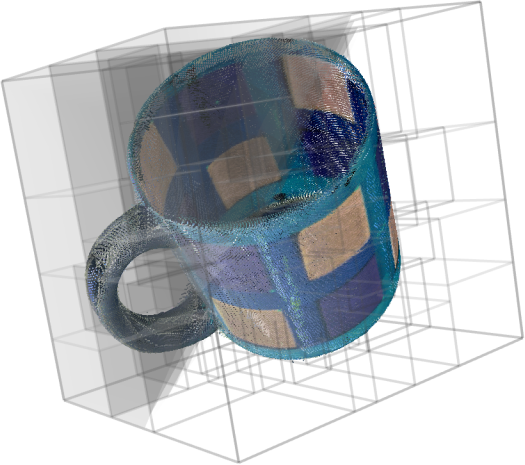
\includegraphics[width=0.45\textwidth]{images/mug}}
    \end{picture}
\end{frame}
%%==================================================================S
\section{Datos Abiertos}
%%==================================================================F 
\begin{frame}
  \frametitle{¡Datos LIBRES!}
  \begin{enumerate}
    \item \beamergotobutton{\url{http://www.lidar-online.com/products-list.php}}
    \item \beamergotobutton{\url{http://opentopo.sdsc.edu/gridsphere/gridsphere?cid=databases}}
    \item \beamergotobutton{\url{http://opentopography.org/}}
    \item \beamergotobutton{\url{http://liblas.org/samples/}}
    \item \beamergotobutton{\url{http://www.csc.noaa.gov/digitalcoast/data/chartstopobathy/download}}
    \item \beamergotobutton{\url{ftp://ftp.lmic.state.mn.us/pub/data/elevation/lidar/}}
  \end{enumerate}
      Muchos más en:
  \begin{enumerate}
    \item \beamergotobutton{\url{http://laszip.org/}}
  \end{enumerate}
\end{frame}
%%==================================================================F 
\begin{frame}
  \frametitle{Descarga de .LAZ}
  \begin{minipage}{0.35\textwidth}
  \begin{enumerate}[<+->]
    \item Open Topography
    \item Minnesota DNR
  \end{enumerate}
  \end{minipage}
    \begin{picture}(375,120)
    \uncover<1->{\put(170,-10){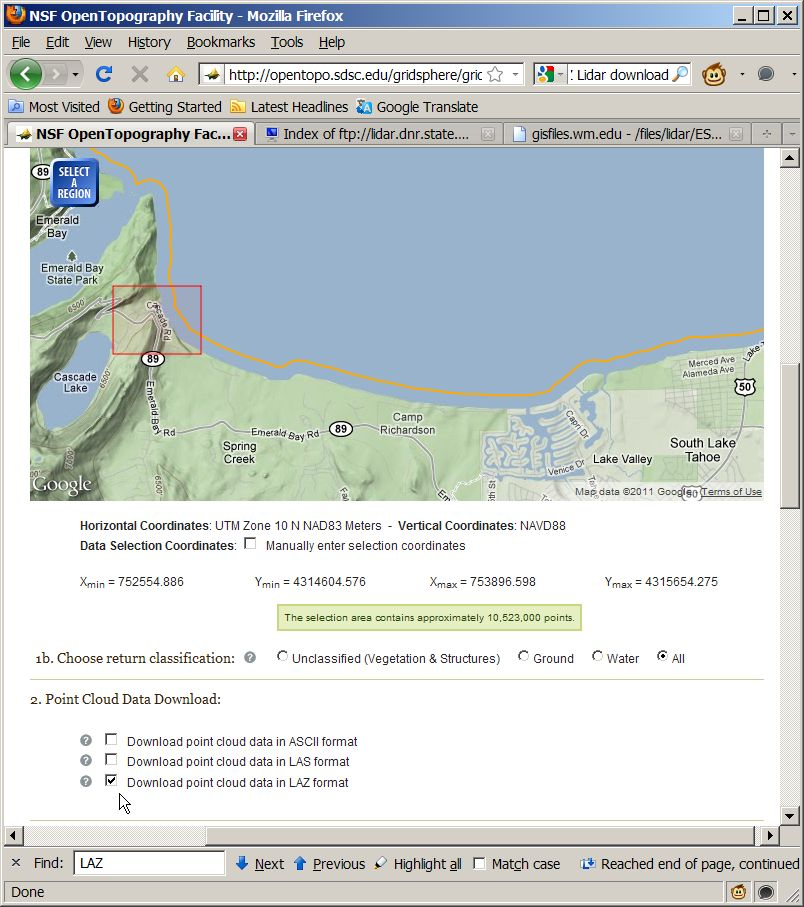
\includegraphics[width=0.48\textwidth]{images/open_topo}}}
    \uncover<2->{\put(170,-10){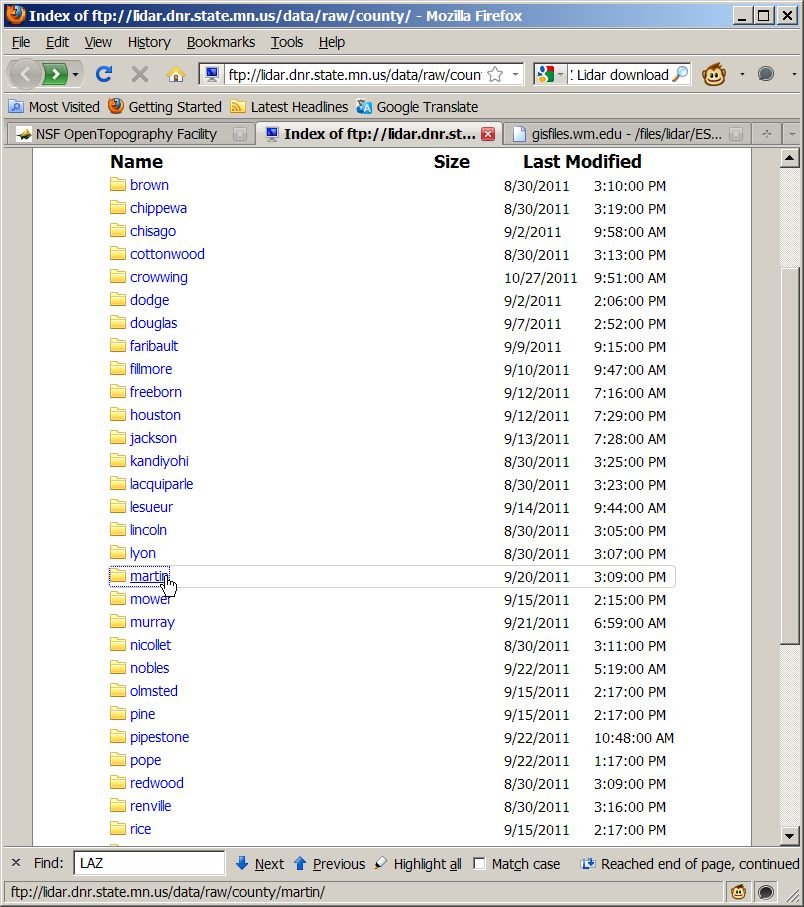
\includegraphics[width=0.48\textwidth]{images/minnesota}}}
    \uncover<3->{\put(170,-10){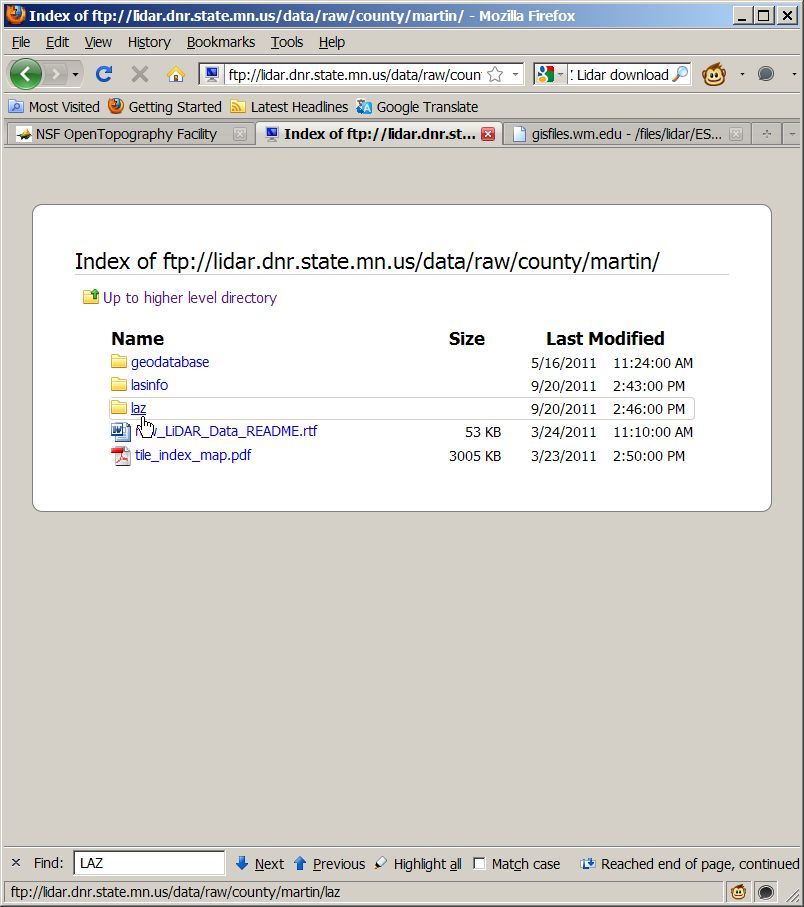
\includegraphics[width=0.48\textwidth]{images/minnesota_martin}}}
    \uncover<4->{\put(170,-10){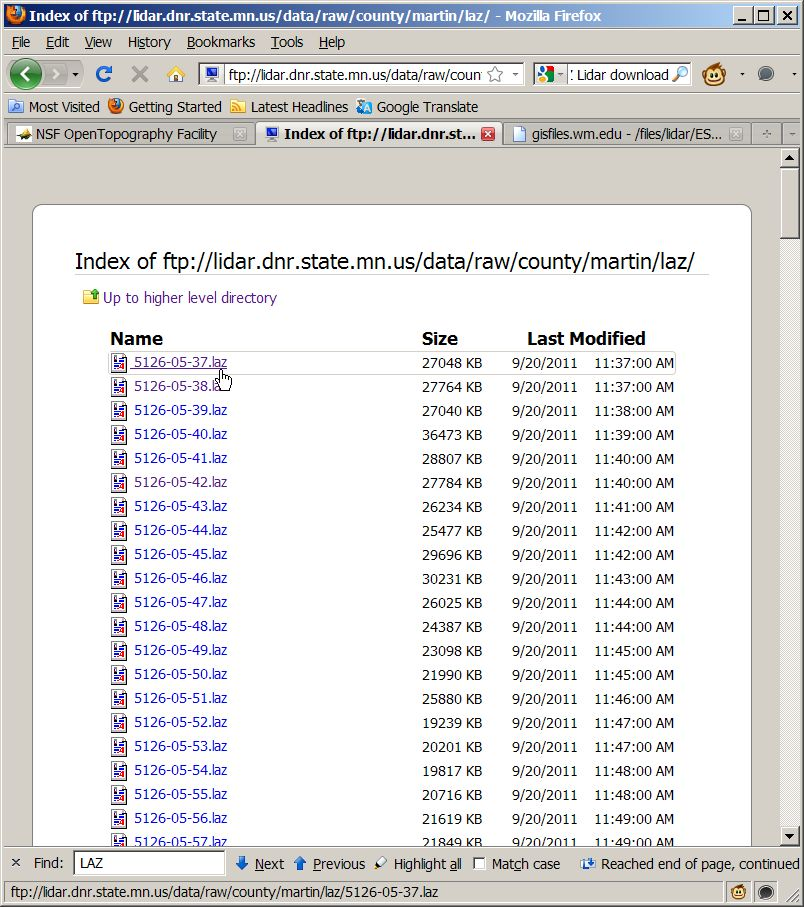
\includegraphics[width=0.48\textwidth]{images/minnesota_laz}}}
    \end{picture}
\end{frame}
%%==================================================================F
\againframe{portada}
%%==================================================================F

%\section{Resumen}
